\documentclass{article.cls}

\usepackage[german]{babel}

\usepackage[letterpaper,top=2cm,bottom=2cm,left=3cm,right=3cm,marginparwidth=1.75cm]{geometry}

\usepackage{amsmath}
\usepackage{graphicx}
\usepackage[colorlinks=true, allcolors=blue]{hyperref}

\title{Übungsprotokoll - NWT2 - Übung 03}
\author{\vspace{0.5cm} \Large VLANS\\ Thomas Brandstätter (s2210239002) & Jakob Mayr (s2210239021)}

\begin{document}
    \maketitle

    \section{Konfiguration der Endsysteme}
    In der folgenden Übung haben wir die PCs 4.1 und 4.2 benutzt, somit sind die Netze 4.x verwendet worden. Die IP-Konfiguration wird folgendermaßen vergeben: Klick auf „Network“ in der Taskleiste -> „Network & Internet Settings“ -> „Change adapter options“ -> gewünschtes Netzwerk Interface auswählen, in diesem Fall Ethernet 2 -> „Properties“ -> Doppelklick auf „Internet Protocol Version 4“ bzw. „Internet Protocol Version 6“. In den geöffneten Fenstern können wir nun jeweils die IP-Adresse, Subnetzmakse/Präfix und das Gateway eingeben. Folglich sind die Konfigurationen beider PC's zu sehen:

    \begin{figure}[ht]
        \centering
        \subfigure[pc41_IPv4_config]{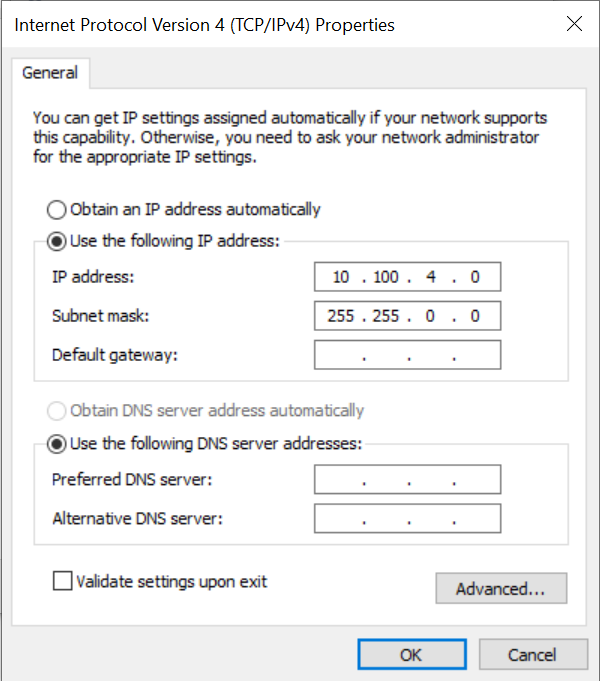
\includegraphics[width=0.2\textwidth]{Arbeitsergebnisse/pc41/pc41_IPv4_config.png}}
        \subfigure[pc41_IPv6_config]{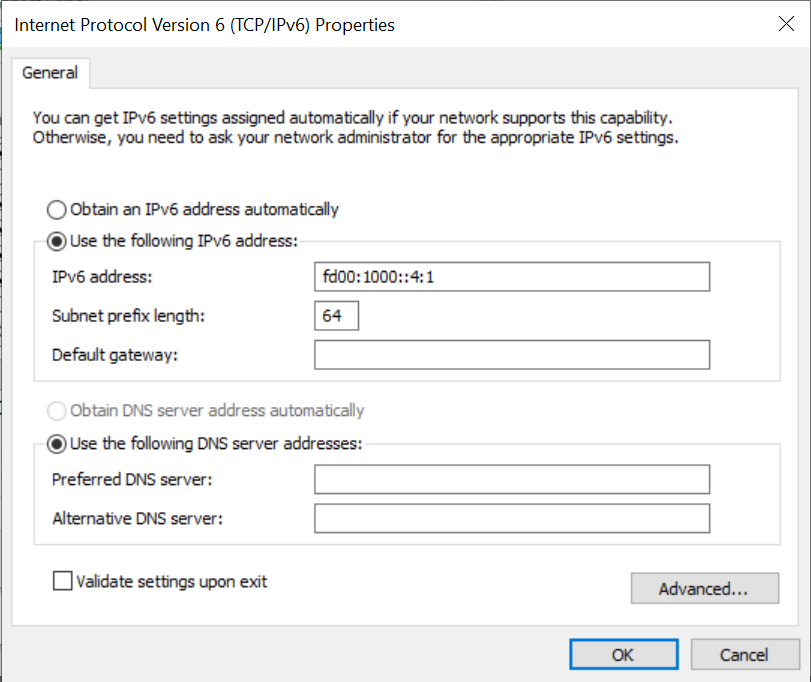
\includegraphics[width=0.2\textwidth]{Arbeitsergebnisse/pc41/pc41_IPv6_config.png}}
        \subfigure[pc42_IPv4_config]{\includegraphics[width=0.2\textwidth]{Arbeitsergebnisse/pc42/pc42_IPv4_config.png}}
        \subfigure[pc42_IPv6_config]{\includegraphics[width=0.2\textwidth]{Arbeitsergebnisse/pc42/pc42_IPv6_config.png}}
        \caption{Konfiguration der Endsysteme}
        \label{fig:four_images}
    \end{figure}

    \section{Konfiguration der Gruppenswitchtes}

    ...

    \subsection{Konfiguration der Gruppenrouter}

    ...

    \subsection{Fragen zur Konfiguration}

    ...

    \subsection{Tests und Interpretation ihrer Resultate}

    ...

    \subsection{Konfiguration}


\end{document}